\section{Model Introduction}

Reinforcement Learning is a new branch and paradigm in the Machine Learning field. But different than the classical Supervised Learning, in RL there is no supervisor, only a reward signal. In this sense, we have an agent which interacts with the environment and receives instant rewards. Therefore, in RL, we can say that the agent's actions affect the subsequent data it receives, and that time really matters, since this data is sequential non i.i.d, and moreover, the total feedback, given by the sum of all rewards, is delayed, not instantaneous \cite{Sutton1998}. All these features make RL a quite unique research field, and it can also finds a wide range of applications, from playing board games to machines control.

The basic model for a RL approach makes use of a discrete state space for representing the agent's state $S_t$, its actions $A_t$ and its full or partial environment observations $O_t$. Thus, at each timestep $t$, the agent receives an observation $O_t$, takes an action $A_t$ and ends up in the next state $S_{t+1}$, receiving an scalar reward $R_{t+1}$. Therefore, the agent's final goal is to maximize the total future reward it gets. Figure \ref{fig:RL_basic_model} illustrates this dynamics representation.

\begin{figure}[H]
    \centering
    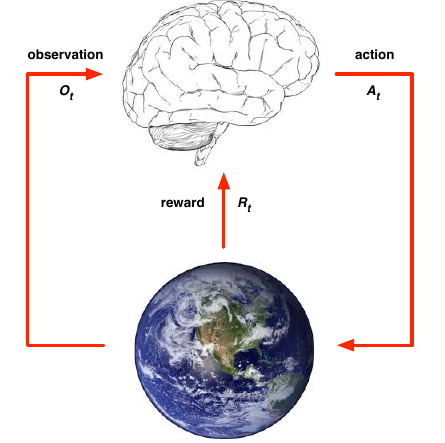
\includegraphics[width=0.4\textwidth]{Chapter2/RL_basic_model.png} 
    \caption{Agent interacting with environment.}
    \label{fig:RL_basic_model}
\end{figure}


\section{Markov Decision Processes}

A classic formal description of an environment for reinforcement learning makes use of Markov decision processes, which inherits the Markov Property from the well known Markov chains. The Markov property establish that the state of the agent captures all the relevant information from the history, in other words, the probability update function only depends of the immediate previous state, as described in \ref{eq:markov_basic}.

\begin{equation}
P(S_{t+1} | S_t) = P(S_{t+1} \mid S_1, ..., S_t)
\label{eq:markov_basic}
\end{equation}

Markov decision processes, however, has a little more complete definition, it is a Markov process with rewards and actions. Basically, can be represented as a tuple $<\textbf{S}, \textbf{A}, P, R, \gamma>$, with each component defined as follows:
\begin{itemize}
\item
	$\textbf{S}$ is a finite set of states the agent can assume in the environment.
\item
	$\textbf{A}$ is a finite set of actions the agent can take.
\item
	$P$ is a state transition probability function, represented as $P_{ss'}^a = \mathbb{P}[S_{t+1}=s' \mid S_t = s, A_t = a]$
\item
	$R$ is a reward function, given by $R_s^a = \mathbb{E}[R_{t+1} \mid S_t = s, A_t = a]$
\item
	$\gamma$ is a discount factor, such that $\gamma \in [0,1]$, used to compute the cumulative total reward.
	
\end{itemize}

Besides this basic tuple representation, there are four more concepts very used in the RL literature that we must present.

\begin{itemize}
\item
	The \textbf{return} $G_T$ is the total discounted reward from time-step t, given by:
	\begin{equation}
	G_t = R_{t+1} + \gamma R_{t+2} + ... = \sum_{k=0}^{\infty}{\gamma^k R_{t+k+1}}
	\end{equation}
	Notice that by introducing the discount factor $\gamma$, it is possible to set the agent preference between short-term and long-term rewards.
\item
	The \textbf{policy} $\pi(a \mid s)$ is a probability distribution function over actions given states, defined by:
	\begin{equation}
	\pi(a \mid s) = \mathbb{P}[A_t=a | S_t=s]
	\end{equation}
	The policy fully defines the behavior of the an agent, and can also be deterministic.
\item
	The \textbf{state-value function} $v_{\pi}(s)$ is the expected return starting from state $s$ and then following a policy $\pi$.
	\begin{equation}
	v_{\pi}(s) = \mathbb{E}_{\pi}[G_t \mid S_t = s]
	\end{equation}
	In informal words, it is a measure of how good the current agent's state is.
\item
	The \textbf{action-value function} $q_{\pi}(s,a)$ is the expected return starting from state $s$, taking action $a$, and then following policy $\pi$
	\begin{equation}
	q_{\pi}(s,a) = \mathbb{E}_{\pi}(G_t \mid S_t = s, A_t = a)
	\end{equation}
	It can be understood as a measure of how good it is to take a given action at the agent's current state.
\end{itemize}

\section{RL Algorithms}

\subsection{Categorizing RL}

\subsection{Value Function Methods}

\subsection{Policy Search Methods}